\section{Experimental Results}
In order to evaluate our method, we perform artifact correction and motor imagery classification through the pipeline illustrated in \cref{fig:pipeline} on the BCI Competition IV dataset 2a \citep{brunner2008bci}. The dataset contains 4-class motor imagery EEG data from 9 subjects. Each subject participated in two sessions of 6 runs on different days. The training data is from the first session, and the test data is from the second. A run consist of 48 labeled trials, divided evenly between the 4 classes. Each trial measured the brain signals of a subject on 22 EEG channels and 3 EOG channels. We disregard the EOG channels since we are interested in correcting artifacts without any reference signals. Examples of trials, channels, runs, and sessions are shown in \cref{fig:dataset}. What we refer to as a trial is three second span (750 samples) of motor imagery, i.e., without the cue, break, etc. in between.

\begin{figure*}
	\centering
	\begin{adjustbox}{width=\textwidth}
		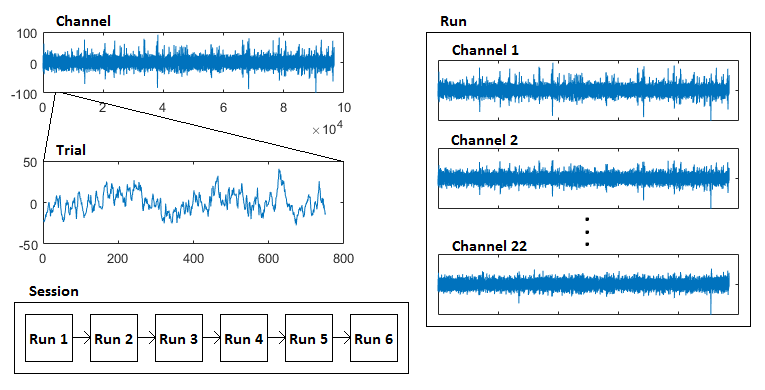
\includegraphics{figures/bciiv2a.png}
	\end{adjustbox}
	\caption{Sessions, runs, channels, trials, and the relations between them.}
	\label{fig:dataset}
\end{figure*}

We set up two pipelines to be compared. The first consists of artifact correction, followed by feature extraction with FBCSP and Random Forest classification. The second pipeline is identical but without the artifact correction step, i.e., just FBCSP and Random Forest. We run Random Forest with six predefined seeds and return the mean to ensure reproducibility. 
To test the generality of the pipeline, we perform 6-fold cross-validation on the training data using five runs for training and one for validation. We run 200 iterations of Bayesian Optimization of select hyperparameters for each pipeline. The best hyperparameters from cross-validation for each pipeline is then used to costruct the pipeline for the final evaluation, where we predict the labels for the test data. We repeat this for each subject. 
\Cref{fig:results} shows the obtained accuracies with and without artifact correction, as well as KAPPA scores for each subject. 

With 200 iterations the artifact correction did not overall yield better results than with no artifact correction and, in fact performed worse on some subjects. One possible cause may be that optimizing 27 parameters over 200 iterations is not a large enough budget to find optimal values for all hyperparameters, since the search space for 27 parameters is much larger than the search space for the 2 parameters optimized in the pipeline with no artifact correction. For this reason, we increased the iterations from 200 to 300 to see if this would yield improved results as illustrated in \cref{fig:i300}. As can be seen, a slight increase on some subjects but decreases in accuracy on other subjects. This indicates, that 300 iterations are still not enough to optimize over such a large search space. \todo{discuss in discussion that this may also indicate that we need more trials/folds for each subject to obtain better generality}

Because our objective is to determine if removing the artifact signal from the raw signal yields improvements in classification accuracy, we manually set the non-artifact correction parameters to the best obtained values found in the non-correction evaluations, instead of further increasing the number of iterations. Consequently,this introduces the assumption that we have found the optimal (or close to) values of the non-correction parameters through bayesian optimization. Therefore, we now optimize the $\theta$ parameters to find the values that yield the highest accuracy. The results of running 200 iterations with this assumption are shown in \cref{fig:fixed-params}. \todo{discuss these results when we get them}

To determine the significance of these results we use the Wilcoxon signed-rank test. \Cref{fig:wilcoxon} shows the results of the test.

\begin{table}[H]
	\centering
	\caption{Wilcoxon signed-rank test}
	\label{fig:wilcoxon}
	\begin{tabular}{@{}l|llll@{}}
		\toprule
		S & No OACL & OACL & Diff & Rank \\ \midrule
		1 &   83,04            &                 &      &      \\
		2 &   57,18            &                 &      &      \\
		3 &   78,18            &                 &      &      \\
		4 &   65,74            &                 &      &      \\
		5 &   58,85            &                 &      &      \\
		6 &   50,23            &                 &      &      \\
		7 &   68,75            &                 &      &      \\
		8 &   74,54            &                 &      &      \\
		9 &   75,64            &                 &      &      \\ \bottomrule
	\end{tabular}
\end{table}

\subsection{Discussion}\label{sec:discussion}
\todo{discuss that optimal filterbank ranges are different from subject to subject}
In the original OACL paper by \citep{li2015ocular}, the relative heights ranges specified in \cref{eq:ranges} were determined by manual inspection of the characteristics of ocular artifacts. Since we generalized this as an optimization of hyperparameter, the found ranges are no longer guaranteed to be optimal in regards to ocular artifacts, but instead optimized for correcting the noise that most negatively affects the classification results. In fact, since we optimize the ranges for maximal classification accuracy, the method may be removing parts of the signal that are technically not artifacts, but removing them increases the performance of the classification model.

Moreover, we have run the Bayesian optimization with the default settings with regards to exploration vs. exploitation. Since running experiments on the pipeline with OACL is relatively expensive, it would be better to tune the Bayesian optimization to spend more time on selecting the best candidate future sample to perform the next experiment on. Additionally, using a different kernel would likely improve the results \citep{snoek2012practical}.

As explained in \cite{hoffmann2008correction}, residual artifacts were still present after noise reduction methods were applied. We have also observed that residual artifacts are present, this can be seen in \cref{fig:oacl-signals}, where an event is registered around $x \approx 170$, but the following desynchronization/synchronization is not registered. A way that this could be handled is to always check if a residual artifact is present when an artifact is registered that, and mark it. These signals might need a separate $\theta$, since the signature of these artifacts is quite different from the artifacts introduced by eye blinks.
